% ------------------------------------------------------------------------------
% TYPO3 Version 9.3 - What's New - Chapter "Changes for Integrators" (German Version)
%
% @author	Michael Schams <schams.net>
% @license	Creative Commons BY-NC-SA 3.0
% @link		http://typo3.org/download/release-notes/whats-new/
% @language	German
% ------------------------------------------------------------------------------
% LTXE-CHAPTER-UID:		3a9852ea-e2360d9d-1ff5eec1-a7de3f9f
% LTXE-CHAPTER-NAME:	Changes for Integrators
% ------------------------------------------------------------------------------

\section{Änderungen für Integratoren}
\begin{frame}[fragile]
	\frametitle{Änderungen für Integratoren}

	\begin{center}\huge{Kapitel 2:}\end{center}
	\begin{center}\huge{\color{typo3darkgrey}\textbf{Änderungen für Integratoren}}\end{center}

\end{frame}

% ------------------------------------------------------------------------------
% LTXE-SLIDE-START
% LTXE-SLIDE-UID:		0e80eecb-f66842d4-e73c50c8-c2bb58a6
% LTXE-SLIDE-TITLE:		...
% LTXE-SLIDE-REFERENCE:	#84843 - Use no-cookie domain for youtube by default
% ------------------------------------------------------------------------------

\begin{frame}[fragile]
	\frametitle{Änderungen für Integratoren}
	\framesubtitle{No-Cookie-Domain für YouTube-Videos}

	% decrease font size for code listing
	\lstset{basicstyle=\smaller\ttfamily}

	\begin{itemize}
		\item Youtube-Videos werden standardmäßig über die No-Cookie-Domain
			\url{https://www.youtube-nocookie.com} gerendert
		\item Die reguläre Domain \texttt{www.youtube.com} kann bei Bedarf durch folgende
			TypoScript-Konfiguration erzwungen werden:

			\begin{lstlisting}
				lib.contentElement {
				  settings {
				    media {
				      additionalConfig {
				        no-cookie = 0
				      }
				    }
				  }
				}
			\end{lstlisting}

	\end{itemize}

\end{frame}

% ------------------------------------------------------------------------------
% LTXE-SLIDE-START
% LTXE-SLIDE-UID:		0e80eecb-f66842d4-e73c50c8-c2bb58a6
% LTXE-SLIDE-TITLE:		General Data Protection Regulation
% LTXE-SLIDE-REFERENCE:	#84843 - Use no-cookie domain for youtube by default
% LTXE-SLIDE-REFERENCE:	GDPR Initiative: https://forge.typo3.org/issues/84776
% ------------------------------------------------------------------------------

\begin{frame}[fragile]
	\frametitle{Änderungen für Integratoren}
	\framesubtitle{Datenschutz-Grundverordnung}

	\begin{itemize}
		\item  Um IP-Adressen mehrerer Datenbanktabellen nach bestimmter Zeit zu anonymisieren,
			kann der Scheduler-Task aktiviert werden.\newline

			Zum Beispiel die Tabelle \texttt{sys\_log}, nach 30 Tagen:
			\begin{figure}
				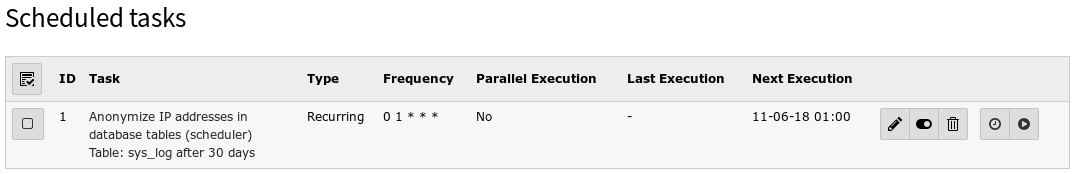
\includegraphics[width=1\linewidth]{ChangesForIntegrators/IpAnonymizationSchedulerTask.png}
			\end{figure}

		\item Der \href{https://typo3.com/blog/tag/gdpr/}{TYPO3 GmbH Blog}
			enthält weitere Informationen zur DSGVO
	\end{itemize}

\end{frame}

% ------------------------------------------------------------------------------
% LTXE-SLIDE-START
% LTXE-SLIDE-UID:		0e80eecb-f66842d4-e73c50c8-c2bb58a6
% LTXE-SLIDE-TITLE:		FE/BE User Accounts and Passwords
% LTXE-SLIDE-REFERENCE:	#85026 - salted passwords changes
% ------------------------------------------------------------------------------

\begin{frame}[fragile]
	\frametitle{Änderungen für Integratoren}
	\framesubtitle{FE/BE Benutzerkonten und Passwörter}

	% decrease font size for code listing
	\lstset{basicstyle=\tiny\ttfamily}

	\begin{itemize}
		\item Unverschlüsselte-Passwörter sind für BE/FE-Benutzer nicht mehr möglich
		\item Inaktive FE/BE Benutzerdatensätze können aus der Datenbank entfernt werden, indem der Schedular-Task
			"Table garbage collection task" hinzugefügt wird und "Clean all available tables"
			aktiviert wird\newline
			\smaller
				(Daten die nicht existieren können im Falle einer Sicherheitsverletzung nicht
				beeinträchtigt werden)
			\normalsize

			\begin{lstlisting}
				<?php
				$tableGarbageCollectionTask = \TYPO3\CMS\Scheduler\Task\TableGarbageCollectionTask::class;
				$GLOBALS['TYPO3_CONF_VARS']['SC_OPTIONS']['scheduler']['tasks'][$tableGarbageCollectionTask]
				  ['options']['tables'] = [
				  'be_users' => [
				    'dateField' => 'lastlogin',
				    'expirePeriod' => 30
				  ]
				];
			\end{lstlisting}

		\item Siehe \href{https://docs.typo3.org/typo3cms/extensions/scheduler/Installation/BaseTasks/Index.html}{die Dokumentation} für weitere Informationen
	\end{itemize}
\end{frame}

% ------------------------------------------------------------------------------
% LTXE-SLIDE-START
% LTXE-SLIDE-UID:		f38ee3cb-51d1aa0a-4f6884bf-adadc9e3
% LTXE-SLIDE-TITLE:		"Duplicate" Button
% LTXE-SLIDE-REFERENCE:	#84749 - Hide "duplicate" button by default
% ------------------------------------------------------------------------------

\begin{frame}[fragile]
	\frametitle{Änderungen für Integratoren}
	\framesubtitle{"Duplicate"-Taste}

	% decrease font size for code listing
	\lstset{basicstyle=\smaller\ttfamily}

	\begin{itemize}
		\item Die Taste zum duplizieren eines Inhaltelements ist jetzt standardmäßg ausgeblendet
		\item Die Sichtbarkeit kann durch TSconfig ("1" = enabled) aktiviert werden:

			\begin{lstlisting}
				options.showDuplicate = 1
				options.showDuplicate.[table] = 1
			\end{lstlisting}

	\end{itemize}
	\vspace{-0.5cm}
	\begin{figure}
		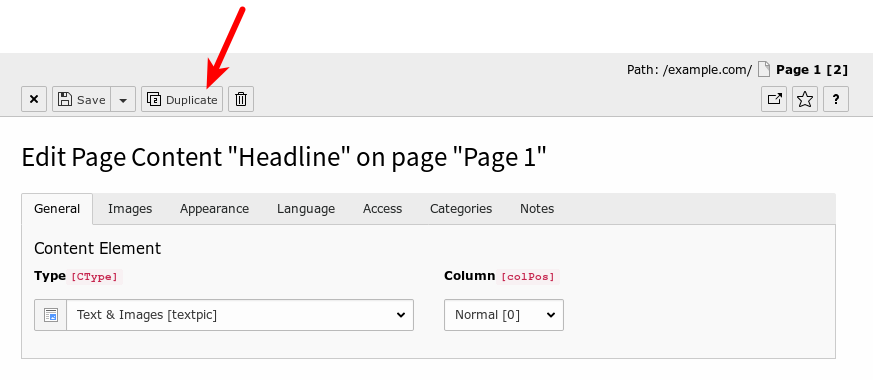
\includegraphics[width=0.8\linewidth]{ChangesForIntegrators/DuplicateButtonHiddenByDefault.png}
	\end{figure}

\end{frame}

% ------------------------------------------------------------------------------
% LTXE-SLIDE-START
% LTXE-SLIDE-UID:		0e80eecb-f66842d4-e73c50c8-c2bb58a6
% LTXE-SLIDE-TITLE:		HTML5 Date Form Element
% LTXE-SLIDE-REFERENCE:	#82511 - EXT:form add HTML5 date form element
% ------------------------------------------------------------------------------

\begin{frame}[fragile]
	\frametitle{Änderungen für Integratoren}
	\framesubtitle{\texttt{EXT:form} HTML5 Formularelement: Datum}

	% decrease font size for code listing
	\lstset{basicstyle=\tiny\ttfamily}

	\begin{itemize}
		\item Das Formularframework enthält ein neues Formularelement "\texttt{Date}",
			dazu gehört auch ein passender Validator
		\item Dies ist technisch ein HTML5 \texttt{'type=date'} Attribut
			(siehe \href{https://www.w3.org/TR/2011/WD-html-markup-20110405/input.date.html}{w3c.org})
		\item Ein Beispiel dafür (beinhaltet auch einen "DateRange" Validator):

			\begin{lstlisting}
				type: Date
				identifier: date-1
				label: Date
				defaultValue: '2018-03-02'
				properties:
				  displayFormat: 'd.m.Y'
				  fluidAdditionalAttributes:
				    min: '2018-03-01'
				    max: '2018-03-30'
				    step: '1'
				validators:
				  -
				    identifier: DateRange
				    options:
				      minimum: '2018-03-01'
				      maximum: '2018-03-30'
			\end{lstlisting}

	\end{itemize}

\end{frame}

% ------------------------------------------------------------------------------
% LTXE-SLIDE-START
% LTXE-SLIDE-UID:		0e80eecb-f66842d4-e73c50c8-c2bb58a6
% LTXE-SLIDE-TITLE:		Destructive Database Schema Changes
% LTXE-SLIDE-REFERENCE:	#85160 - Non destructive database schema changes in extension manager
% ------------------------------------------------------------------------------

\begin{frame}[fragile]
	\frametitle{Änderungen für Integratoren}
	\framesubtitle{Änderungen im Bezug auf destruktive Datenbankstruktur}

	\begin{itemize}
		\item Wenn eine Extension über den Extension-Manager installiert oder aktualisiert wird
			und \textit{destruktive} Datenbankänderungen erforderlich sind, werden diese Änderungen
			nicht automatisch angewendet
		\item "Destruktive" Änderungen sind zum Beispiel Änderungen von bestehenden Spalten, 
			Entfernen einer Spalte, Index- oder Tabellendefinition usw.
		\item Um diese besonderen Datenbank-Updates zu überprüfen und möglicherweise auszuführen
			gehen Sie bitte  in ADMIN TOOLS → Maintenance → Analyze Database Structure\newline
	\end{itemize}

	\vspace{-0.4cm}

	% Translators: remove the illustration below, if it does not fit on the
	% slide, e.g. in case your language requires more space. The illustration is
	% not really required, just "nice to have".

	\begin{figure}
		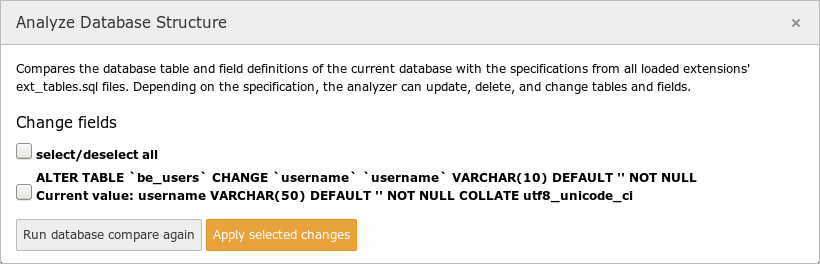
\includegraphics[width=0.6\linewidth]{ChangesForIntegrators/DestructiveDatabaseChanges.png}
	\end{figure}

\end{frame}

% ------------------------------------------------------------------------------
% LTXE-SLIDE-START
% LTXE-SLIDE-UID:		0e80eecb-f66842d4-e73c50c8-c2bb58a6
% LTXE-SLIDE-TITLE:		TypoScript Conditions
% LTXE-SLIDE-REFERENCE:	#84760 - TypoScript conditions for site and siteLanguage
% ------------------------------------------------------------------------------

\begin{frame}[fragile]
	\frametitle{Änderungen für Integratoren}
	\framesubtitle{TypoScript-Bedienungen}

	Neue TypoScript-Bedienung:

	\begin{itemize}
		\item Bedingung für die Eigenschaften eines Site-Objekts

			\begin{lstlisting}
				[site = identifier = someIdentifier, base = https://example.com/]
				  page.30.value = foo
				[global]
			\end{lstlisting}

		\item Bedingung für die Seitensprache

			\begin{lstlisting}
				[siteLanguage = locale = de_CH.UTF-8, title = Switzerland]
				  page.40.value = bar
				[global]
			\end{lstlisting}

	\end{itemize}

\end{frame}

% ------------------------------------------------------------------------------
% LTXE-SLIDE-START
% LTXE-SLIDE-UID:		0e80eecb-f66842d4-e73c50c8-c2bb58a6
% LTXE-SLIDE-TITLE:		HMENU cObj and language IDs
% LTXE-SLIDE-REFERENCE:	#84775 - Extend HMENU to support auto filling of special.value for special=language
% ------------------------------------------------------------------------------

\begin{frame}[fragile]
	\frametitle{Änderungen für Integratoren}
	\framesubtitle{\texttt{HMENU} cObj und Sprachen IDs}

	% decrease font size for code listing
	%\lstset{basicstyle=\tiny\ttfamily}

	\begin{itemize}
		\item \texttt{HMENU} Inhaltsobjekt unterstützt jetzt das automatische Ausfüllen von
			Sprach-IDs für Sprachmenüs

			\begin{lstlisting}
				10 = HMENU
				10 {
				  special = language
				  special.value = auto
				}
  			\end{lstlisting}

	\end{itemize}

\end{frame}

% ------------------------------------------------------------------------------
% LTXE-SLIDE-START
% LTXE-SLIDE-UID:		0e80eecb-f66842d4-e73c50c8-c2bb58a6
% LTXE-SLIDE-TITLE:		View User TSConfig Data
% LTXE-SLIDE-REFERENCE:	#85017 - User TSConfig shown in Configuration module
% ------------------------------------------------------------------------------

\begin{frame}[fragile]
	\frametitle{Änderungen für Integratoren}
	\framesubtitle{User TSconfig Daten anzeigen}

	User TSConfig Daten des aktuell angemeldeten Benutzers können unter  
	\textbf{System -> Configuration} gefunden werden

	\begin{figure}
		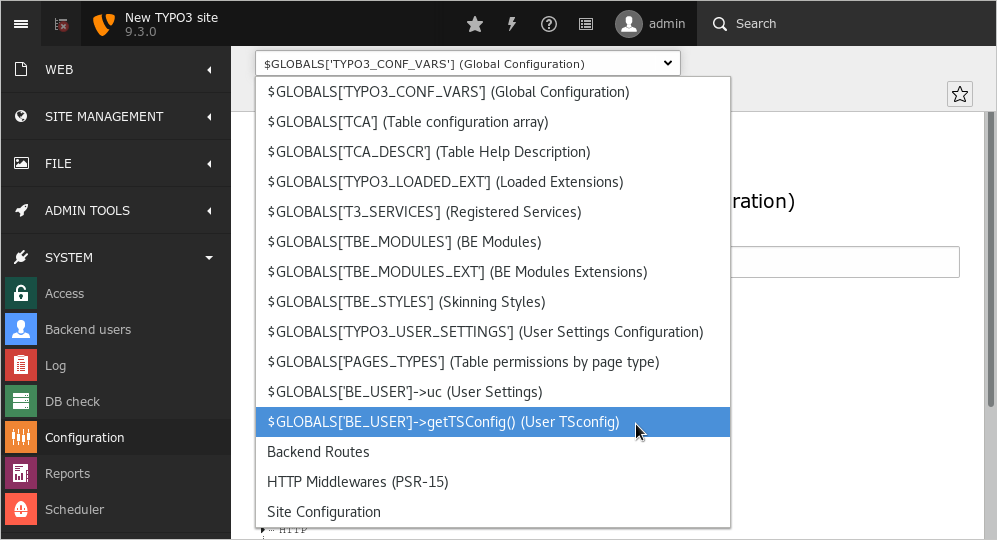
\includegraphics[width=0.75\linewidth]{ChangesForIntegrators/SystemConfigurationUserTSConfig.png}
	\end{figure}

\end{frame}

% ------------------------------------------------------------------------------
% LTXE-SLIDE-START
% LTXE-SLIDE-UID:		0e80eecb-f66842d4-e73c50c8-c2bb58a6
% LTXE-SLIDE-TITLE:		Miscellaneous
% LTXE-SLIDE-REFERENCE:	#69274 - Preserve image rotation if orient is saved in exif
% LTXE-SLIDE-REFERENCE:	#85147 - Render SEO meta tags in frontend
% LTXE-SLIDE-REFERENCE:	#84715 - Set exclude property for tt_content fields
% ------------------------------------------------------------------------------

\begin{frame}[fragile]
	\frametitle{Änderungen für Integratoren}
	\framesubtitle{Sonstiges}

	\begin{itemize}
		\item TYPO3 berücksichtigt beim Bearbeiten des Bildes (z.B. Skalierung/Zuschneiden
			die Bildausrichtung, die als EXIF-Angabe gespeichert wird
		\item SEO-bezogene Meta-Tags, die in den Seiteneigenschaften festgelegt sind,
			werden jetzt standardmäßg im Frontend gerendert
		\item Die \textit{exclude} Eigenschaft ist für folgende Felder festgelegt:

			\begin{itemize}
				\smaller
				\item \texttt{tt\_content.file\_collections}
				\item \texttt{tt\_content.filelink\_size}
				\item \texttt{tt\_content.filelink\_sorting}
				\item \texttt{tt\_content.filelink\_sorting\_direction}
			\end{itemize}

			\small
				Dalls Redakteure diese Felder bearbeiten dürfen, müssen die Zugriffberechtigungen 
				angepasst werden!
			\normalsize

	\end{itemize}

\end{frame}

% ------------------------------------------------------------------------------
